% Figure from MATH 556 notes, section 41 (Step 3: a ball about the origin). From the board sketch (Lecture 16).
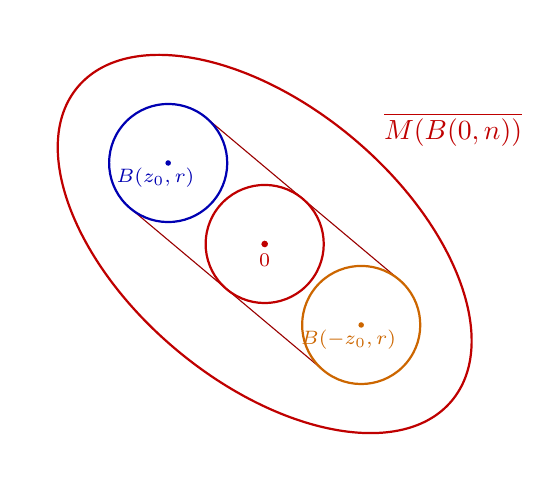
\begin{tikzpicture}[scale=1.0, >=stealth, rotate=-40]
    \draw[thick, red!75!black] (0,0) ellipse (3.1 and 1.75);
    \node[red!75!black] at (0.9,2.65) {$\overline{M(B(0,n))}$};
    \draw[red!60!black, thin] (-1.6,0.75) -- (1.6,0.75);
    \draw[red!60!black, thin] (-1.6,-0.75) -- (1.6,-0.75);
    \draw[thick, blue!70!black] (-1.6,0) circle (0.75);
    \fill[blue!70!black] (-1.6,0) circle (1pt);
    \node[blue!70!black, font=\scriptsize] at (-1.6,-0.25) {$B(z_0, r)$};
    \draw[thick, orange!80!black] (1.6,0) circle (0.75);
    \fill[orange!80!black] (1.6,0) circle (1pt);
    \node[orange!80!black, font=\scriptsize] at (1.6,-0.25) {$B(-z_0, r)$};
    \draw[thick, red!75!black] (0,0) circle (0.75);
    \fill[red!75!black] (0,0) circle (1.2pt) node[below, font=\scriptsize] {$0$};
\end{tikzpicture}
